\documentclass{article} 
\usepackage[utf8]{inputenc} 
\usepackage[spanish]{babel}
\usepackage{graphicx} 
\usepackage{subcaption}
\usepackage{hyperref}
\usepackage{listings}
\usepackage{xcolor}
\usepackage{float}

\definecolor{codegreen}{rgb}{0,0.6,0}
\definecolor{codegray}{rgb}{0.5,0.5,0.5}
\definecolor{codepurple}{rgb}{0.58,0,0.82}
\definecolor{backcolour}{rgb}{0.95,0.95,0.92}

\lstdefinestyle{mystyle}{
    backgroundcolor=\color{backcolour},
    commentstyle=\color{codegreen},
    keywordstyle=\color{blue},
    numberstyle=\tiny\color{codegray},
    stringstyle=\color{codepurple},
    basicstyle=\ttfamily\footnotesize,
    breakatwhitespace=false,
    breaklines=true,
    captionpos=b,
    keepspaces=true,
    numbers=left,
    numbersep=5pt,
    showspaces=false,
    showstringspaces=false,
    showtabs=false,
    tabsize=2
}

\lstdefinelanguage{CSS}{
  keywords={color,background-image:,margin,padding,font,weight,display,position,top,left,right,bottom,list,style,border,size,white,space,min,width, transition:, transform:, transition-property, transition-duration, transition-timing-function},	
  sensitive=true,
  morecomment=[l]{//},
  morecomment=[s]{/*}{*/},
  morestring=[b]',
  morestring=[b]",
  alsoletter={:},
  alsodigit={-}
}
\lstset{style=mystyle}
\date{} 

\begin{document} 

\begin{center}
    
\includegraphics[width=1\textwidth]{Images/Imagenes Latex/logo/LogoBIASbn.png}\\ 
\end{center}
    
\title{BIAS} 

\vspace{1cm} 

\textbf{Integrantes del Proyecto:} 

\begin{itemize}
    \item Adell, Nicolas Fabian
    \item De Blasi, Luca
    \item Diaz Melion, Danilo Sebastian
    \item Gil Soria, Ian Lucas
    \item Montenegro, Luciano Nahuel
    \item Sojka, Santiago Alejandro
\end{itemize}

\tableofcontents 

\newpage 

\section{Introducción}

BIAS es un módulo aplicable a una silla de ruedas que permite el control mental, permitiendo a los usuarios dirigirla mediante el sus pensamientos, eliminando la necesidad de controles físicos tradicionales y optimizando la experiencia de movilidad. Este proyecto representa un avance significativo en el campo de la movilidad asistida, con el objetivo de mejorar la independencia y la calidad de vida de las personas con movilidad reducida.

Este sistema se basa en la avanzada tecnología de interfaz cerebro-computadora (BCI), la cual captura las señales neuronales del usuario y las traduce en comandos precisos para maniobrar la silla de ruedas sin esfuerzo. Además, el diseño modular y adaptable del sistema permite su integración en diversos modelos de sillas de ruedas y su personalización según las necesidades específicas de cada usuario. 

La seguridad es una prioridad fundamental en este desarrollo, por lo que el módulo incorpora múltiples capas de redundancia y verificación de señales, asegurando que la silla de ruedas responda de manera precisa y confiable a las intenciones del usuario. 

Aspiramos a revolucionar la forma en que las personas con movilidad reducida interactúan con su entorno, brindándoles una herramienta que amplía su capacidad para controlar su vida de manera más segura e independiente.

\subsection{Resumen del proyecto}
Este proyecto se centra en el desarrollo de una silla de ruedas controlada mediante señales cerebrales. El sistema se compone principalmente de los siguientes componentes: la silla de ruedas, un dispositivo EEG (electroencefalograma) y dos motores que permiten al usuario moverse en la dirección deseada.

El funcionamiento del sistema es el siguiente: el usuario se sienta en la silla y se coloca el EEG en la cabeza. A continuación, el usuario piensa en la dirección en la que desea moverse, y los motores responden en consecuencia.

El EEG tiene la función de leer las señales cerebrales del usuario. Estas señales se clasifican en las categorías de alpha, beta, gamma, delta y theta, y luego se someten a un proceso de filtrado para eliminar cualquier ruido. Posteriormente, las señales filtradas son analizadas por una Inteligencia Artificial (IA) desarrollada por nuestro equipo, la cual identifica patrones para determinar si el usuario desea moverse o detenerse.

Además, la silla está equipada con un sistema de emergencia que se activa en caso de lecturas erróneas o la detección de obstáculos. Este sistema de emergencia está compuesto por sensores infrarrojos y ultrasónicos que detectan la presencia de obstáculos frente a la silla.

\subsection{Motivación}
Como estudiantes de séptimo año, buscamos desarrollar un proyecto con el fin de cumplir con el requerimiento horario de practicas profesionalizantes. Nuestra intención inicial fue encontrar el proyecto ideal en cuestiones de impacto social, enfocándonos en la mejora de la calidad de vida de aquellas personas con discapacidades. Bajo este marco, y tras una extensa investigación, proponemos crear un módulo aplicable a una silla de ruedas controlado mediante la actividad cerebral del usuario, utilizando tecnología de interfaces cerebro-computadora (BCI), para brindarles mayor autonomía, independencia y participación social.   Creemos que este proyecto tiene el potencial de transformar la vida de las personas con movilidad motora reducida debido a enfermedades como ELA, esclerosis múltiple o cuadriplejia, permitiéndoles controlar su propio movimiento y mejorar significativamente su calidad de vida.
\subsection{Objetivos}
El objetivo de este proyecto es desarrollar una silla de ruedas motorizada que pueda ser controlada por la actividad cerebral del usuario. Esto beneficiaría a las personas con discapacidades motoras severas para lograr independencia y movilidad, mejorando su calidad de vida y participación en la sociedad. De esta manera, estas personas las cuales no pueden caminar o tienen movilidad reducida, pueden gozar de la utilización de una silla de ruedas controlada por señales cerebrales sin la utilización de ambas manos y meramente por sus pensamientos, dándole libertad y autonomía al usuario.

\section{¿Quiénes somos?}
Somos el grupo BIAS (Brain Intelligence Artificial System), conformado por seis estudiantes de la especialidad de Aviónica del séptimo año, segunda división, comisión " C ", de la Escuela Técnica N° 7 IMPA "Taller Regional Quilmes". Nuestro equipo se encuentra comprometido en el desarrollo de un módulo adaptable para sillas de ruedas, para así poder brindarles mas independencia y movilidad.
\subsection{Contactos}

En este apartado se detallarán los contactos a los integrantes del proyecto, adjuntando enlaces a sus redes:

\subsubsection{Adell Nicolás}

    \href{https://instagram.com/nicolas.adell}{Instagram}

    
    \href{http://www.linkedin.com/in/nicolas-adell-354508297}{LinkedIn}

    
    \href{mailto:nicolas.fabian2005@gmail.com}{Gmail}

\subsubsection{De Blasi Luca}

    \href{https://instagram.com/luca.deblasii}{Instagram}

    
    \href{https://www.linkedin.com/in/luca-de-blasi-31164b304}{LinkedIn}

    
    \href{mailto:luqac2006@gmail.com}{Gmail}

\subsubsection{Diaz Melión Danilo}

    \href{https://instagram.com/_danilodiaz}{Instagram}

    
    \href{https://www.linkedin.com/in/danilodiazmelion/}{LinkedIn}

    
    \href{mailto:danilodiaz934@gmail.com}{Gmail}

\subsubsection{Gil Soria Ian}

    \href{https://instagram.com/ian_gilsooor}{Instagram}

    
    \href{https://www.linkedin.com/in/ian-lucas-gil-soria-a8090b2a8?utm_source=share&utm_campaign=share_via&utm_content=profile&utm_medium=android_app}{LinkedIn}

    
    \href{mailto:ianlucasgilsoria@gmail.com}{Gmail}

\subsubsection{Montenegro Luciano}


    \href{https://instagram.com/luchito_.montenegro}{Instagram}

    
    \href{https://www.linkedin.com/in/luciano-montenegro-3215aa304}{LinkedIn}

    
    \href{mailto:lucianomontenegro1021@gmail.com}{Gmail}



\subsubsection{Sojka Santiago}

    \href{https://instagram.com/sojkaa.sant}{Instagram}

    
    \href{https://www.linkedin.com/in/santiago-sojka-817198271/}{LinkedIn}

    
    \href{mailto:santiagosojka@gmail.com}{Gmail}




\section{Desarrollo del Proyecto}
En este capítulo se expondrá en detalle la metodología empleada para avanzar en el desarrollo del proyecto, incluyendo las fuentes de inspiración y los proyectos similares que se tomaron como referencia para el diseño de nuestros circuitos y la programación de los sistemas. Además, se incluirán imágenes ilustrativas de estos proyectos de referencia, con el fin de ofrecer una comprensión visual más completa. Al finalizar el capítulo, se presentarán y explicarán los resultados obtenidos, evaluando su eficacia en relación con los objetivos planteados.

\subsection{Metodología}
La metodología aplicada en este proyecto se basa en la organización del equipo en dos grupos especializados. El primer grupo se encarga del desarrollo de los programas, siendo ejemplos de esto los filtros virtuales, programas de recepción y procesado, mientras que el segundo se dedica a la implementación de los motores, sistemas de emergencia y filtros. Esta división del trabajo permite una utilización más eficiente del tiempo, al abordar simultáneamente diversas áreas del proyecto, lo que resulta en un avance más significativo en periodos de tiempo más reducidos.


\subsection{Historia del Arte}
En este capitulo se repasa todos los conceptos previamente vistos mediante los cuales pudimos empezar a conceptualizar la idea del proyecto.



\subsubsection{Neuralink}
Uno de los casos que nos permitió aproximarnos a la conceptualización del proyecto fue el chip cerebral estilo implante de Neuralink, denominado Telepathy. Este dispositivo, desarrollado por la compañía de Elon Musk, tiene como objetivo facilitar la vida de las personas mediante la optimización de herramientas y su adaptación al cuerpo humano a través del implante. El chip crea una conexión entre el ser humano y dispositivos electrónicos, permitiendo, por ejemplo, controlar una puerta con traba eléctrica, desbloquear un teléfono móvil, e incluso monitorear el estado de ánimo de las personas.


Este ejemplo nos ofreció una perspectiva sobre la viabilidad de desarrollar un dispositivo, que, aunque no tan complejo, pudiera ser controlado por el propio cuerpo humano. A partir de esta premisa, iniciamos una investigación para explorar las posibilidades y opciones disponibles basadas en esta idea.


\subsubsection{Ryan Lopez EEG}
Si bien nuestro motivo y objetivo principal era crear un dispositivo original e innovador, también nos propusimos investigar proyectos con cierta similitud. En este proceso, encontramos el repositorio de un estudiante que desarrolló un sistema capaz de detectar señales alfa y, en función de las reacciones o pensamientos del usuario, permitir el control a través de un test de concentración. Este test consistía en que el usuario debía mantener un estado de concentración mientras estudiaba un documento para un examen, en lo que se podría considerar un simulacro.


El sistema desarrollado por Ryanlopezz activaba una alarma si los niveles de concentración del usuario comenzaban a disminuir, basándose en un espectro de señales alfa transmitidas por un conjunto de electrodos EEG dorados conectados a la cabeza del estudiante. Además, el sistema realizaba otras dos pruebas: una de ellas consistía en escribir en código Morse mediante pensamientos, enviando "pulsos de concentración", y la otra permitía controlar el movimiento de un personaje en el famoso videojuego "Flappy Bird", ajustando el impulso para subir o bajar.

En el siguiente link se adjunta la página de GitHub de Ryan Lopez en donde se puede observar más a detalle los programas y archivos de su EEG.


\begin{center}
    \href{https://github.com/ryanlopezzzz/EEG}{Ryan Lopez GitHub}
\end{center}


Gracias al mismo proyecto realizado por este usuario, pudimos desarrollar nuestro propio circuito para el sistema de filtrado, ya que íbamos a requerir otras especificaciones con diferentes funciones, tales como la entrada de señal: ya que esta debía ser mayor a la designada, al nosotros trabajar no solo con el espectro radioelectrico de las señales Alpha, sino con las principales señales que el cerebro produce al momento de realizar un pensamiento especifico; Por otro lado nosotros íbamos a requerir no solo un sistema de filtros EEG sino 4 placas del mismo circuito, debido a la posibilidad de maniobrar controlando los 3 ejes de los motores de la silla de ruedas


\begin{center}
    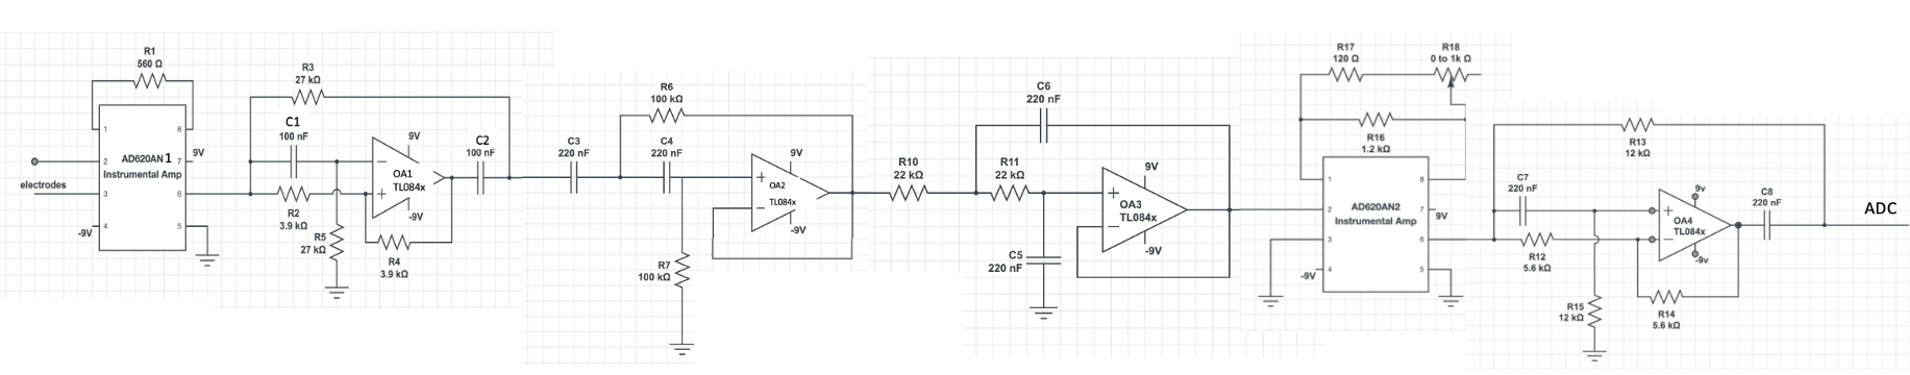
\includegraphics[width=1\textwidth]{Images/Imagenes/filtroeegderyan.png}\\
    
Por otro lado nos dio una primera vista de la localización de los botones EEG como irían colocados en la cabeza

\end{center}

\begin{center}
    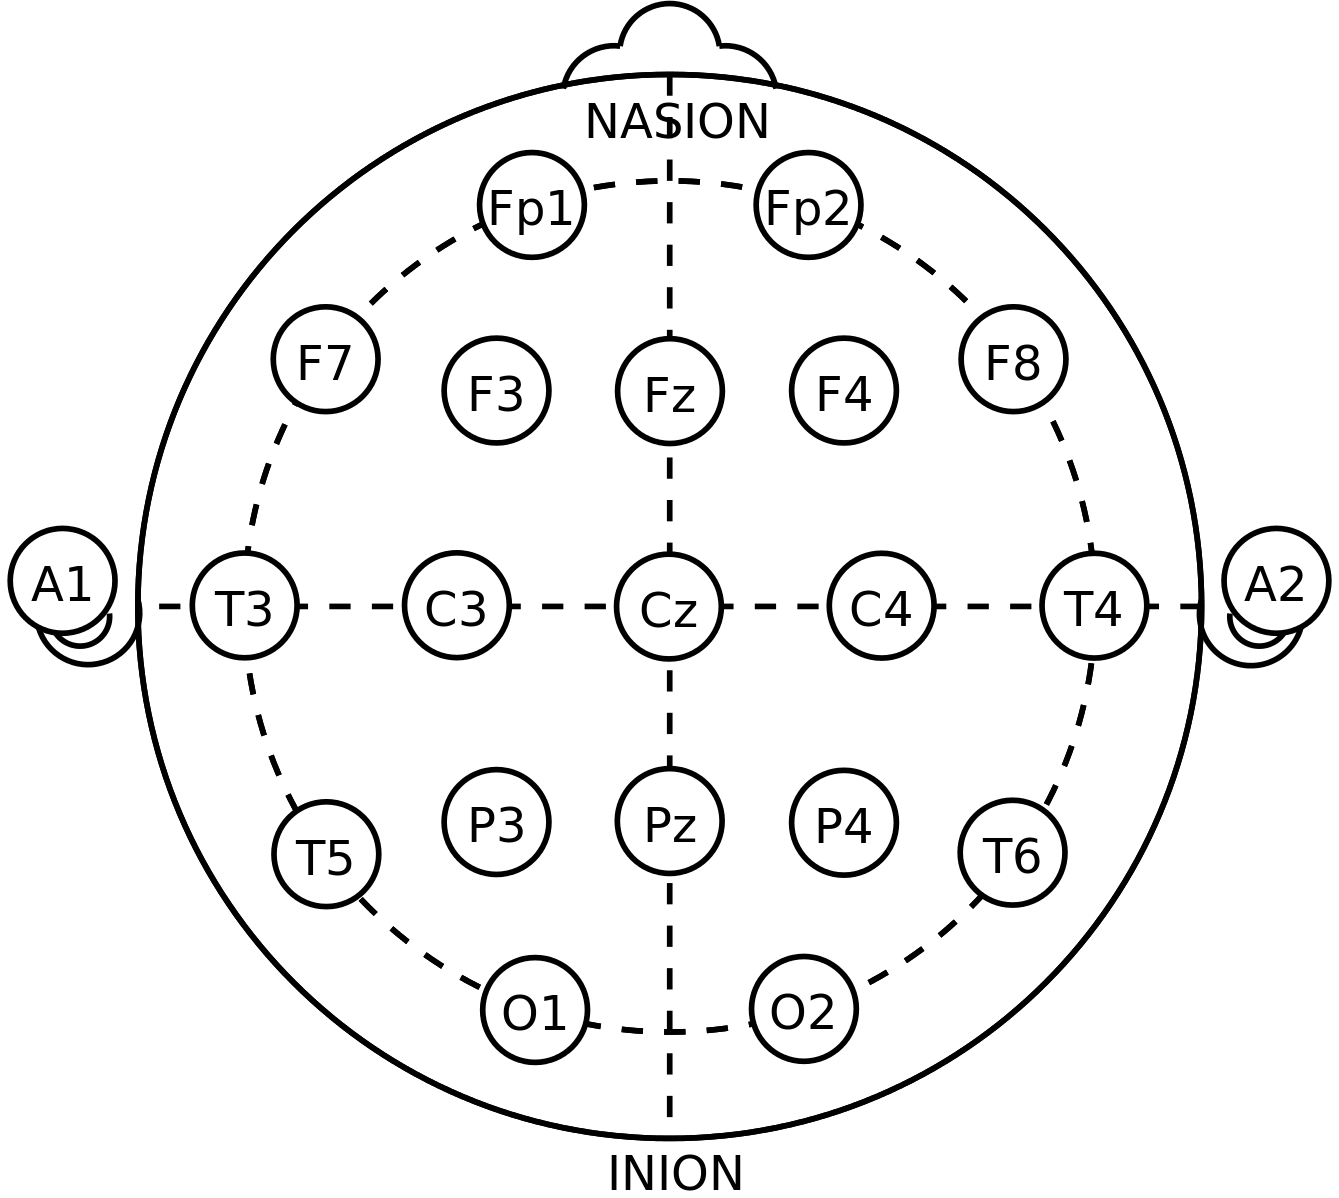
\includegraphics[width=1\textwidth]{Images/Imagenes/localizacionelectrodoseeg.png}\\

\end{center}

Así mismo para el estudio del aérea de medicina y saber como el cerebro humano se encarga de transmitir ciertas señales eléctricas gracias a la actividad cerebral  tuvimos en cuenta los actuales dispositivos de eneflografos, como se componen y actúan gracias ala actividad cerebral, bajo un especto radioelectrico determinado adjunto a la clasificación de las ondas transmitidas por el cerebro humano

\subsubsection{OpenBCI}

En nuestra búsqueda de conexiones para un microcontrolador y formas de desarrollar nuestro propio proyecto, descubrimos un sitio web llamado OpenBCI, una compañía especializada en la creación de dispositivos que integran tecnología con la interfaz del cuerpo humano. Esta empresa ha desarrollado un encefalógrafo casero, proporcionando dimensiones y parámetros estructurales que nos permitieron diseñar nuestra propia vincha/casco. Este dispositivo incorpora electrodos EEG, adaptados a la cabeza del usuario, como parte fundamental de nuestro proyecto "BIAS".

\begin{center}
    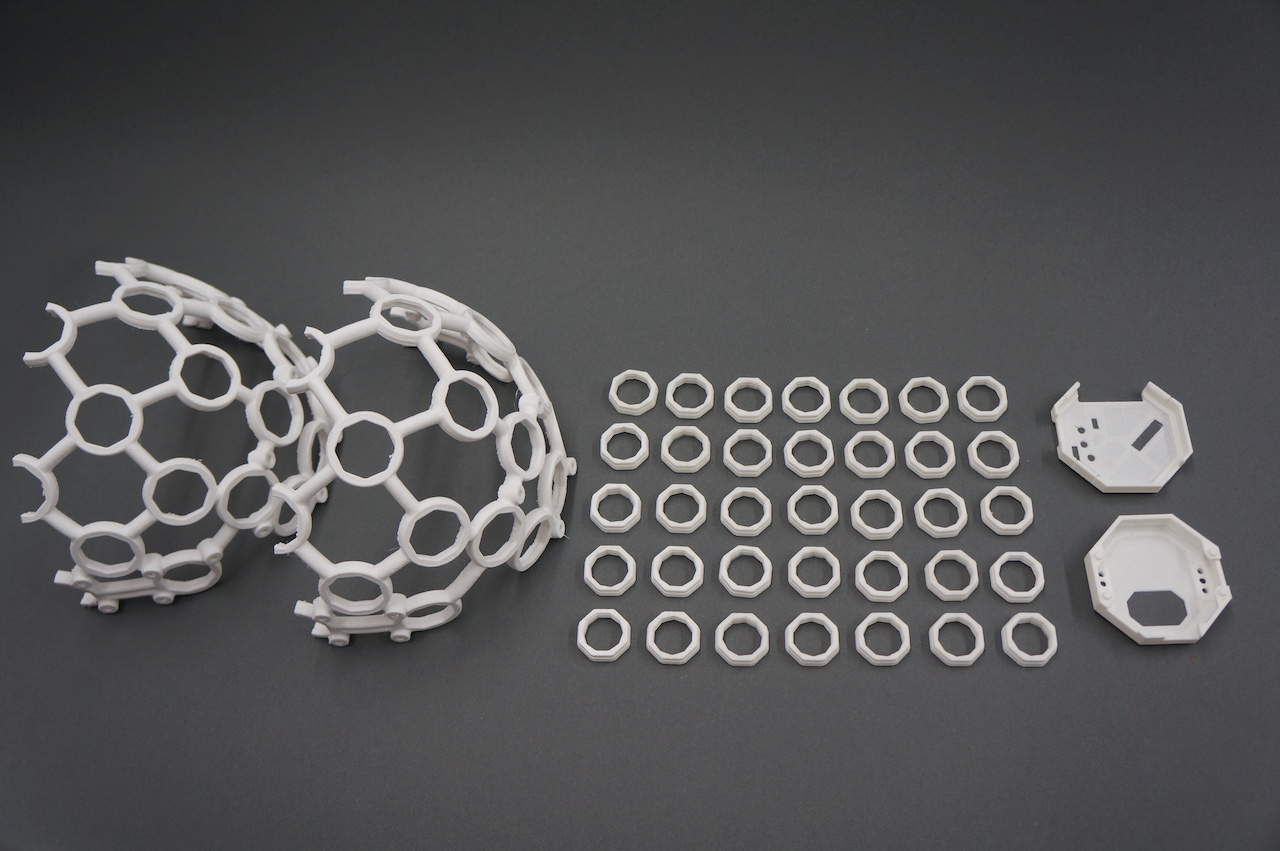
\includegraphics[width=1\textwidth]{Images/Imagenes/vinchamarkiv.png}\\
\end{center}

Además, al ser una compañía especializada en la creación de módulos de microcontroladores, nos proporcionaron orientación en cuanto a cómo realizar las conexiones entre la Raspberry Pi 4 que utilizamos y el sistema de filtrado EEG.

En los siguientes textos se adjuntan enlaces para ver la página oficial de OpenBCI y documentación de referencia correspondiente.

\begin{center}
    \href{https://openbci.com/}{Página oficial de OpenBCI}

    
    \href{https://docs.openbci.com/}{Documentación}

    
\end{center}

\begin{figure}[h!]
\centering

\begin{subfigure}[b]{0.45\linewidth}
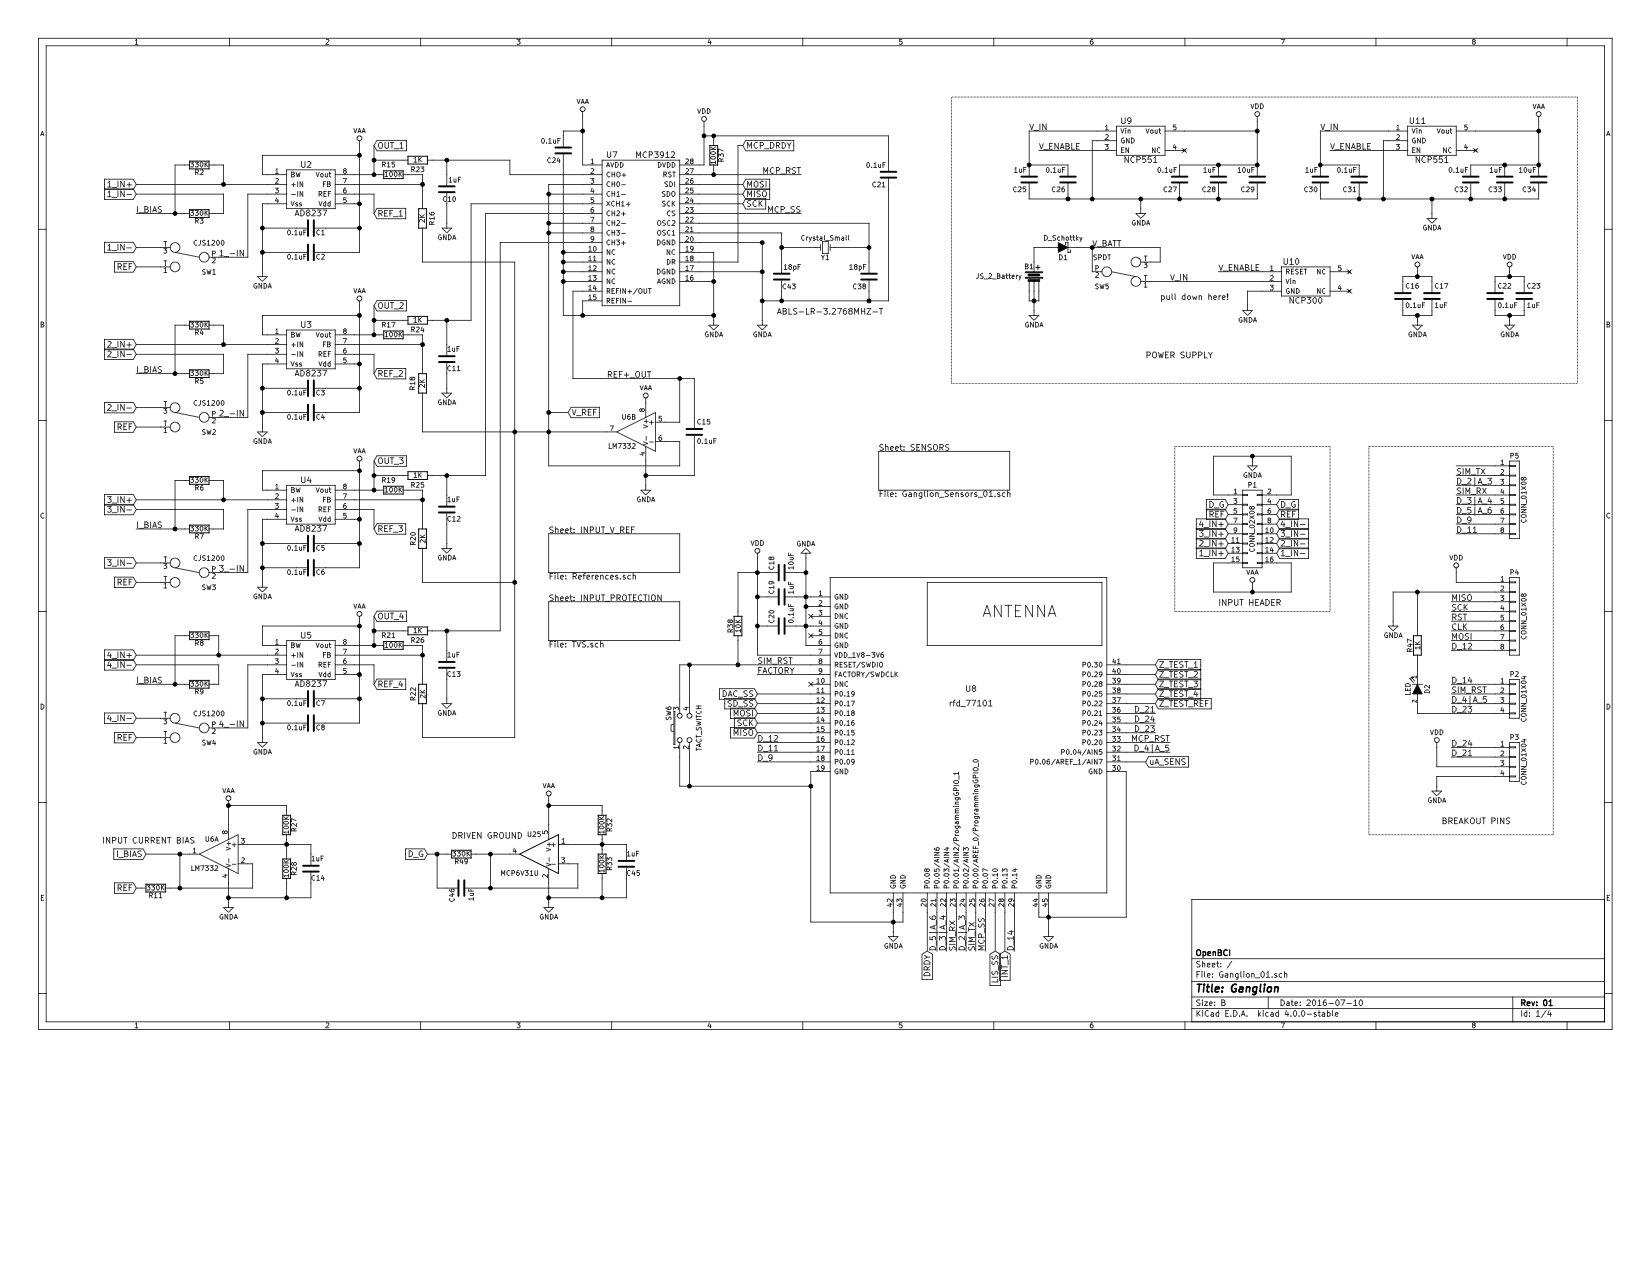
\includegraphics[width=\linewidth]{Images/Imagenes/esquematicodeganglion.png}
\caption{Diseño Esquemático}
\label{fig:westminster_lateral}
\end{subfigure}

\begin{subfigure}[b]{0.45\linewidth}
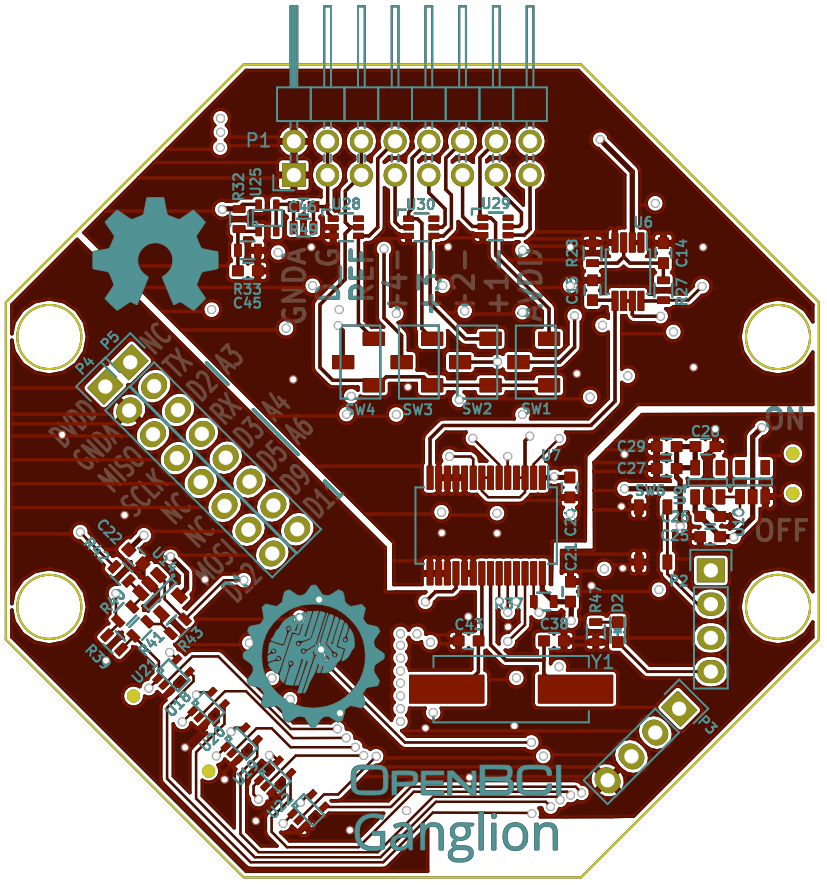
\includegraphics[width=\linewidth]{Images/Imagenes/pcbdeganglion.png}
\caption{DIseño PCB}
\label{fig:westminster_aerea}

\end{subfigure}
\caption{Diseño de microcontrolador de Open BCI}
\label{fig:westminster}
\end{figure}

\begin{center}
    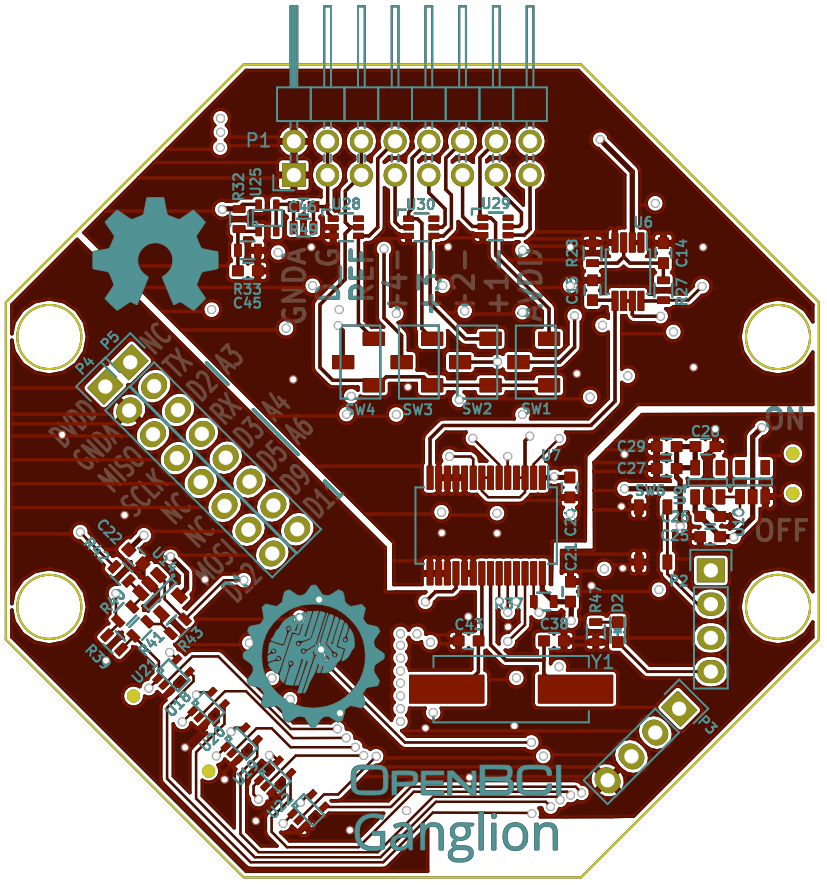
\includegraphics[width=1\textwidth]{Images/Imagenes/pcbdeganglion.png}\\

    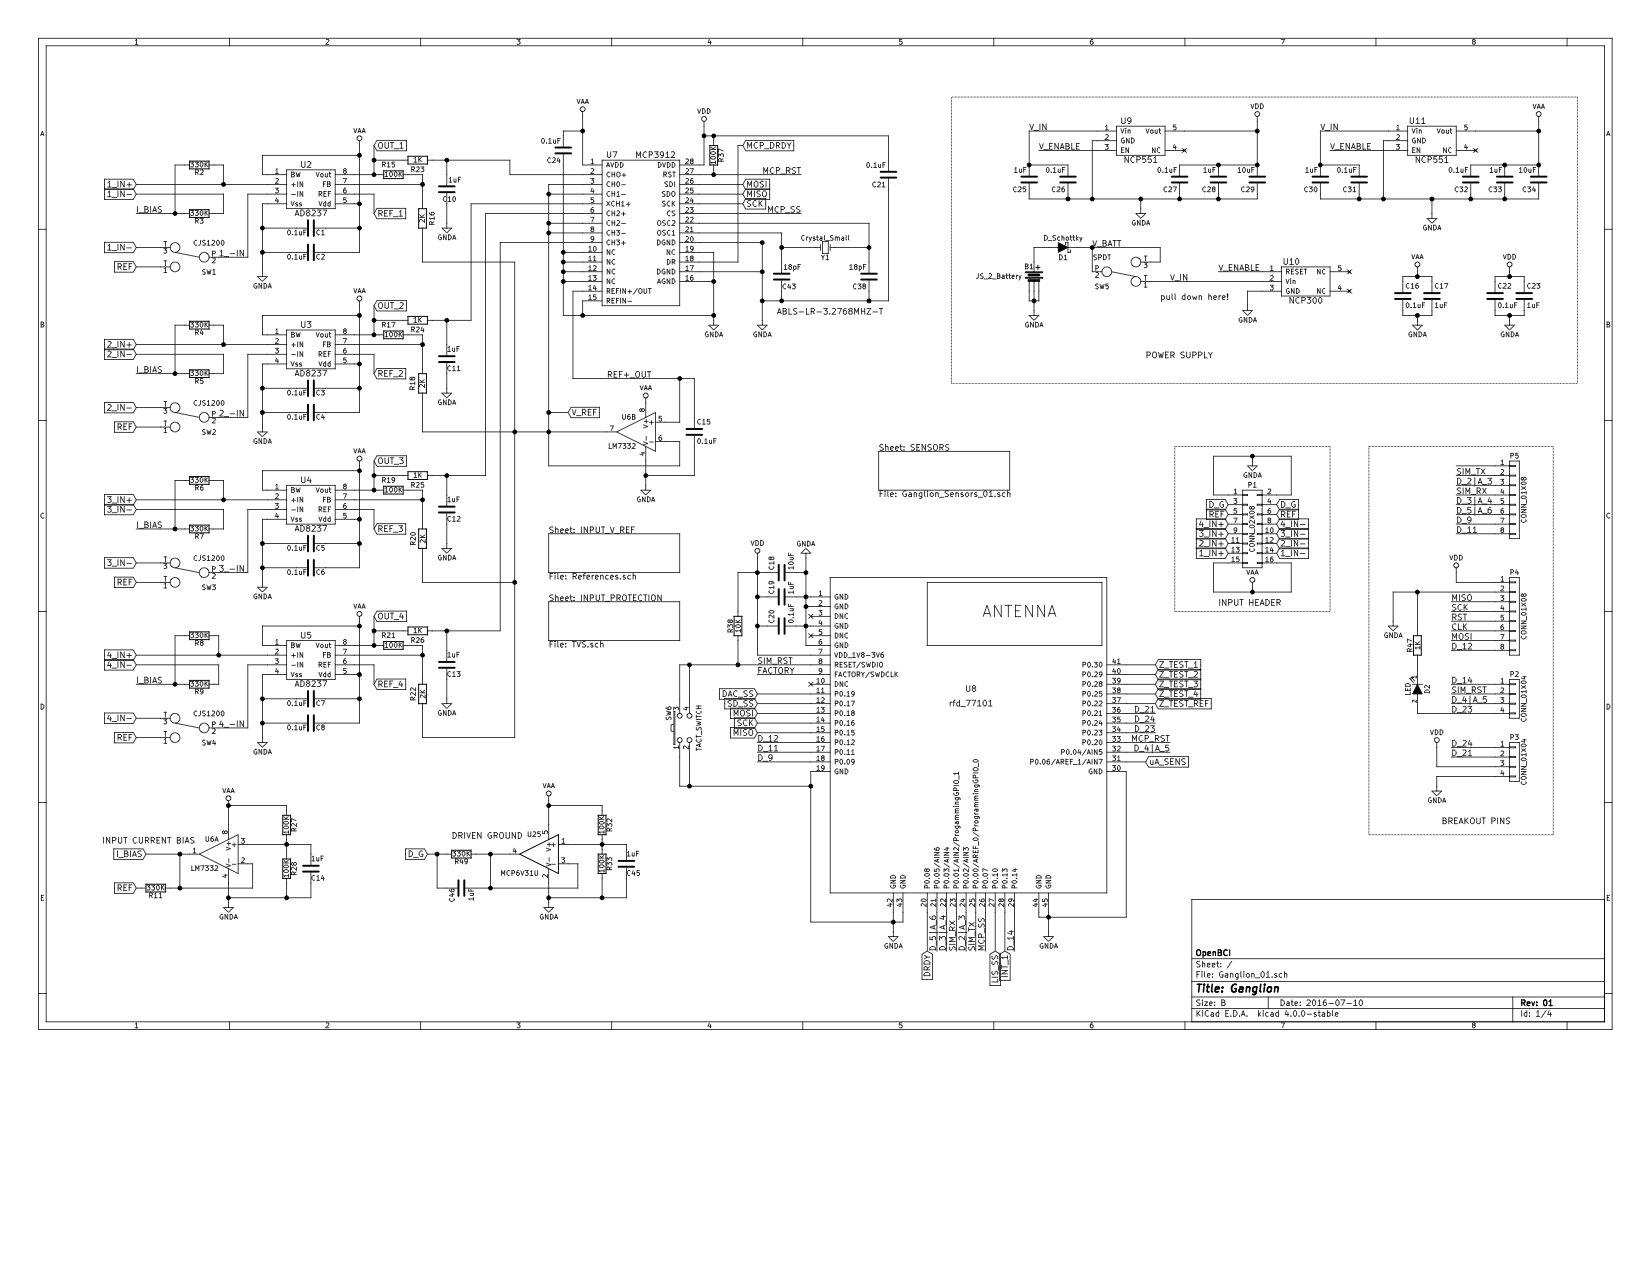
\includegraphics[width=1\textwidth]{Images/Imagenes/esquematicodeganglion.png}\\
\end {center}

\section{Desarrollo Teórico}
En este capítulo se describirán y desarrollarán todos los aspectos teóricos relacionados, justificando la elección de los componentes utilizados. Se abordarán teorías como la Jaula de Faraday y el sistema 10-20, además de ofrecer una explicación detallada sobre los tipos de señales empleadas, entre otros temas relevantes.

\subsection{Distinción de alimentaciones}

\subsection{Sistema 10-20}

\subsection{Comunicación UART}

El UART (Universal Asynchronous Receiver-Transmitter) es un periférico de hardware utilizado para la comunicación serie. Su principal función es permitir la transmisión y recepción de datos de manera asíncrona, lo que implica que no requiere de una señal de clock compartida entre el transmisor y el receptor. A continuación, se destacan las características principales de este tipo de comunicación:

\begin{itemize}
    \item Comunicación serie: Los datos se transmiten de forma secuencial, bit a bit, a través de una línea de transmisión (TX) y se reciben mediante una línea de recepción (RX).
    \item Asincronía: Al no utilizar una señal de clock constante, ambos dispositivos deben estar configurados con la misma velocidad de transmisión (tasa de baudios) para asegurar la correcta recepción de los datos.
    \item Formato de datos: Cada paquete de datos transmitido generalmente incluye un bit de inicio (indicando el comienzo de la transmisión), entre 5 y 9 bits de datos, un bit opcional de paridad (para detección de errores), y uno o dos bits de parada.
    \item Velocidad de transmisión: La velocidad de transmisión de la información, conocida como tasa de baudios, se refiere al número de bits transmitidos por segundo.
\end{itemize}

La implementación de la comunicación UART en nuestro proyecto se utiliza para la recepción y procesamiento de señales. Específicamente, en la RP2040 Zero, enviamos las lecturas de los cuatro canales del ADC (Conversor Analógico-Digital) en formato JSON durante un período de tiempo definido y con una frecuencia de muestreo específica a la Raspberry Pi 4.

\subsection{Gráfico de Fourier}
que es
por que la necesitamos
como lo aplicamos
Explicar ondas cerebrales

\subsection{Filtros digitales}

\subsection{Cantidad de canales}

\subsection{Gel conductor}
El gel conductor neutro empleado en los electroencefalogramas (EEG) es una sustancia formulada para optimizar la conductividad eléctrica entre los electrodos y el cuero cabelludo del paciente. Su principal objetivo es minimizar la resistencia entre los electrodos y la piel, garantizando una transmisión eficiente y sin interferencias de las señales eléctricas cerebrales hacia los electrodos. 

\subsubsection{Cómo aplicar el gel conductor}
En los electrodos de copa dorada, el procedimiento consiste únicamente en rellenar la cavidad de la copa con el gel conductor, posteriormente colocarlo sobre una zona del cuero cabelludo previamente limpiada con algodón, mantenerlo en posición durante unos segundos y eliminar cualquier exceso de gel, en caso de haberlo, con un pequeño trozo de papel. Utilizamos este gel en el proyecto con el fin de obtener la mejor calidad posible en las señales, además de generar un leve efecto de succión que contribuye a mantener los electrodos firmemente adheridos.

\subsection{Jaula de Faraday}
Una jaula de Faraday es, esencialmente, una estructura metálica diseñada para proteger su interior de los campos eléctricos estáticos. Su nombre proviene del físico Michael Faraday, quien construyó la primera de estas estructuras en 1836. Las jaulas de Faraday se utilizan para proteger su contenido de descargas eléctricas y del ruido electromagnético, debido a que, en su interior, el campo eléctrico es nulo. Su principio de funcionamiento se basa en las propiedades de un conductor en equilibrio electrostático, lo que impide que cualquier carga eléctrica atraviese la estructura. Por esta razón, se emplean para proteger dispositivos sensibles a las cargas eléctricas. Este fenómeno es conocido como apantallamiento eléctrico.

\subsubsection{¿Por qué utilizamos una Jaula de Faraday?}
Dado que trabajamos con señales altamente susceptibles al ruido debido a su frecuencia y voltaje, como es el caso de las señales captadas por el EEG, es fundamental mantenerlas lo más aisladas posible de interferencias externas. Además, contamos con una fuente importante de ruido electromagnético: el motor. Por esta razón, es esencial posicionar los componentes lo más alejados posible entre sí y utilizar una Jaula de Faraday en la sección destinada a la recepción y procesamiento de las señales.

La implementación de este elemento se realiza mediante una caja metálica que será ubicada en la parte superior trasera de la silla de ruedas, es decir, en la zona de apoyo de la espalda, para mantenerla lo más distante posible de los motores.

\subsection{Utilización de offsets}

\subsection{Sistema de emergencia}

\subsection{Tipos de alimentaciones}

\subsection{Sistema de control}

\subsection{Puentes H}
Un Puente H es un circuito utilizado para invertir el sentido de giro de un motor y para separar su etapa de potencia con la de control. Su nombre viene de la forma gráfica que tiene el circuito. Se construye con 4 interruptores, pueden ser mecánicos o transistores. En la siguiente imágen se puede ver la forma de un puente H.

\begin{figure}[H]
    \centering
    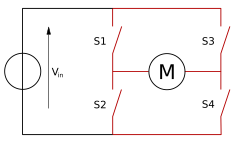
\includegraphics[width=0.5\linewidth]{Images/PuenteH/H_bridge.svg.png}
    \caption{Puente H Genérico por medio de llaves mecánicas}
\end{figure}

En este ejemplo, cuando la llave S1 y S4 se cierran, correrá corriente por esta rama, haciendo que el motor funcione y tenga un sentido de giro. Cuando la llave S2 y S3 se cierran, correrá corriente por esta rama también, pero con sentido de giro invertido. En este circuito, S1 y S2 nunca pueden estar cerradas al mismo tiempo, porque esto generaría un corto circuito, lo mismo con las llaves S3 y S4.

\begin{figure}[H]
    \centering
    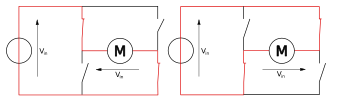
\includegraphics[width=0.70\linewidth]{Images/PuenteH/H_bridge_operating.svg.png}
    \caption{Puente H Operando}
\end{figure}

\subsubsection{Puente H de potencia}
Un puente H de potencia es un tipo de circuito en el que la etapa de potencia, que incluye el motor, los transistores y está conectada a altas tensiones y corrientes, se encuentra separada de la etapa de control, la cual generalmente opera con voltajes más bajos. Esta separación se realiza para proteger la etapa de control de las altas tensiones, que podrían dañar o quemar sus circuitos. Podemos utilizar nuestro puente H como ejemplo para ilustrar este concepto:

 \begin{figure}[H]
     \centering
     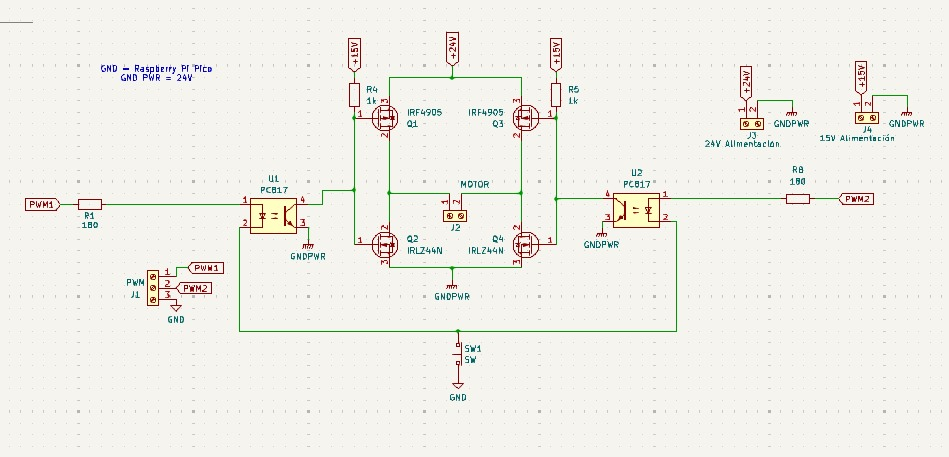
\includegraphics[width=0.85\linewidth]{Images/PuenteH/WhatsApp Image 2024-08-28 at 9.05.56 AM.jpeg}
     \caption{Nuestro Puente H de potencia}
     \label{fig:enter-label}
 \end{figure}

En nuestro puente H, hemos separado las ramas del motor de las de control, ya que el motor opera con 24V DC y tiene una corriente eficaz de 3,5A. Para controlar el motor de manera eficiente, hemos optado por un diseño que incluye cuatro transistores MOSFET de potencia, los cuales pueden soportar picos de hasta 74A y 82A, garantizando que puedan manejar la corriente del motor de manera continua. Además, los transistores son controlados mediante señales PWM, las cuales atraviesan un optoacoplador para minimizar el riesgo de que la corriente del motor regrese a la placa de control y cause daños. De ésta manera, podemos controlar el giro del motor de manera segura y regulada.


\subsection{Sistema de recepción de señales}

\subsection{Control por PWM}
La modulación por ancho de pulso (PWM, por sus siglas en inglés Pulse Width Modulation) es una técnica empleada para regular la cantidad de energía suministrada a una carga, como un motor o un LED, mediante la variación del ciclo de trabajo de una señal pulsante. En lugar de modificar el voltaje de forma continua, PWM ajusta el tiempo durante el cual la señal permanece en estado alto (encendida) y bajo (apagada) dentro de un período fijo. Esto depende de los siguientes parámetros:


Frecuencia: Se refiere a la cantidad de ciclos de encendido y apagado que ocurren en un segundo, y se mide en Hertz (Hz).


Ciclo de trabajo: Es el porcentaje de tiempo que la señal se mantiene en estado alto durante un ciclo. Por ejemplo:

Un ciclo de trabajo del 0\% implica que la señal está siempre apagada.

Un ciclo de trabajo del 50\% significa que la señal está encendida la mitad del tiempo y apagada la otra mitad.

Un ciclo de trabajo del 100\% indica que la señal permanece siempre encendida.


En nuestro proyecto, aplicamos la técnica de PWM en el control de los motores. Dado que utilizamos dos motores, si estos operaran a su máxima potencia, la silla de ruedas se desplazaría a una velocidad excesiva. Por esta razón, empleamos un ciclo de trabajo del 25\% para limitar la velocidad de avance.



\section{Desarrollo Tecnico}
En este capítulo se proporcionará una descripción detallada sobre el funcionamiento de los distintos circuitos que conforman el dispositivo, así como su interacción en conjunto para cumplir con los objetivos del proyecto. Se explicará de manera clara y concisa cómo se utiliza el dispositivo, incluyendo instrucciones específicas para su correcto manejo y operatividad.

Además, se incluirán datos técnicos relevantes, tales como especificaciones de los componentes, características del diseño, y cualquier otro detalle que sea esencial para la comprensión del sistema. También se abordarán aspectos importantes acerca de las partes constitutivas del dispositivo, su función dentro del esquema general, y las consideraciones necesarias para su mantenimiento y optimización.

\subsection{Descripcion del funcionamiento}
El usuario se sienta en la silla de ruedas y se coloca el dispositivo EEG. El EEG capta las señales cerebrales (alfa, beta, gamma, delta y theta) y las somete a un proceso de filtrado por hardware que incluye un filtro notch de 50 Hz, un filtro pasa-bajo de 100 Hz, un filtro pasa-alto de 0,5 Hz y un segundo filtro notch de 50 Hz. Posteriormente, las señales pasan por un circuito de compensación de offset para poder realizar la lectura por parte de la RP2040 Zero ya que la misma no puede leer valores negativos. Esta unidad se encarga de leer los datos mediante cuatro canales de ADC y enviarlos a la Raspberry Pi 4 por protocolo UART, donde se aloja el programa principal para el funcionamiento de la silla de ruedas.

Entre estos códigos se encuentran el control de motores, los filtros digitales, el procesamiento de señales y la inteligencia artificial (IA). Una vez las señales llegan a la Raspberry Pi 4, se filtran digitalmente para eliminar el ruido y mejorar la calidad de los datos. Tras el filtrado, las señales se envían a la IA, que tiene la función de reconocer los patrones cerebrales y determinar la dirección en la que el usuario desea moverse. Una vez el patrón ha sido identificado, se envía una señal a los motores para dirigir la silla hacia la dirección deseada (adelante, atrás, izquierda o derecha).

Además, el proyecto incluye un sistema de emergencia diseñado para garantizar la seguridad del usuario. Este sistema se activa si se detecta un error en la lectura de las señales o si hay un obstáculo en la trayectoria deseada. Su objetivo es prevenir accidentes y aumentar la seguridad del usuario al utilizar la silla de ruedas.

El sistema de emergencia utiliza sensores de ultrasonido para detectar la presencia de objetos a menos de 20 cm de la silla. En caso de detección, el sistema frena los motores y activa un LED en la dirección del objeto, además de un buzzer que emite una señal sonora durante un breve período para alertar al usuario sobre la activación del sistema.

\subsubsection{Funcionamiento del EEG}


\subsubsection{Funcionamiento de los filtros HardWare}


\subsubsection{Funcionamiento de los filtros digitales}


\subsubsection{Funcionamiento del Puente H}


\subsubsection{Funcionamiento del Sistema de Emergencia}



\section{Circuitos usados}
En este capítulo se incluirán imágenes de los esquemas de los circuitos, junto con su representación gráfica en formato virtual de los circuitos impresos, así como fotografías de los circuitos completos una vez finalizados.


\subsubsection{Esquemáticos de los filtros}
\begin{figure}[H]
    \centering
    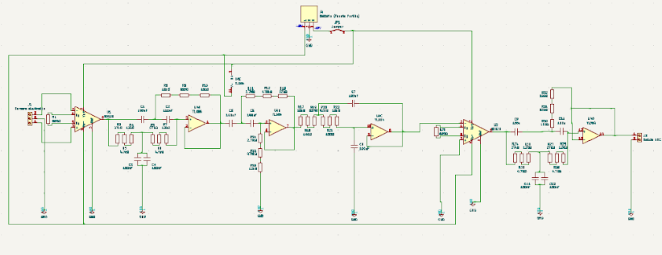
\includegraphics[width=0.5\linewidth]{Images/Filtros/filtroseeg.png}
    \caption{Esquemáticos de los filtros del EEG}
\end{figure}[]

\subsubsection{Esquemáticos del sistema de control}
\begin{figure}[H]
    \centering
    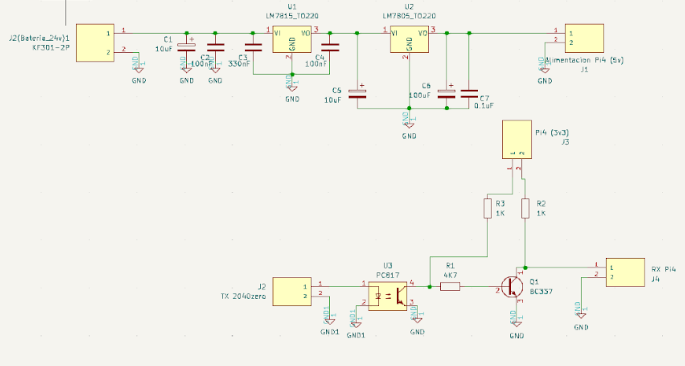
\includegraphics[width=0.5\linewidth]{Images/SistemaControl/sistemadecontrol.png}
    \caption{Esquemáticos del sistema de control}
\end{figure}[]

\subsubsection{Esquemáticos del sistema Offset}
\begin{figure}[H]
    \centering
    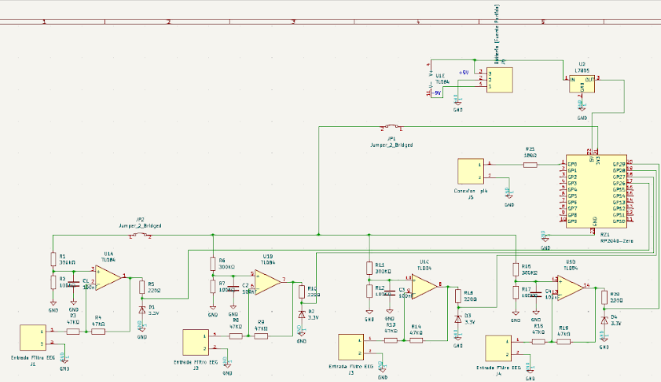
\includegraphics[width=0.95\linewidth]{Images/SistemaOffset/sistemaoffset.png}
    \caption{Esquemático del sistema de Offset}
\end{figure}

\subsubsection{Esquemáticos de los Puentes H}
\begin{figure}[H]
    \centering
     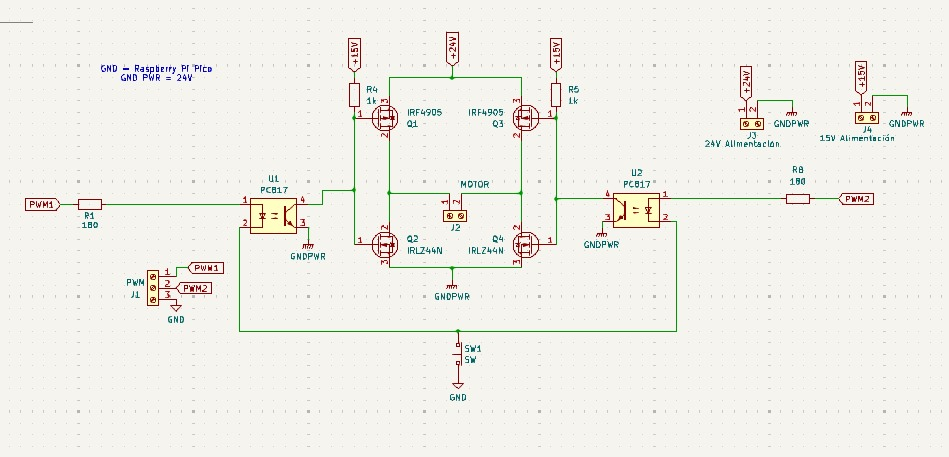
\includegraphics[width=1\textwidth]{Images/PuenteH/WhatsApp Image 2024-08-28 at 9.05.56 AM.jpeg}
    \caption{Puente H (Un Motor)}
\end{figure}

\subsubsection{Esquemático del sistema de emergencia}
\begin{figure}[H]
    \centering
    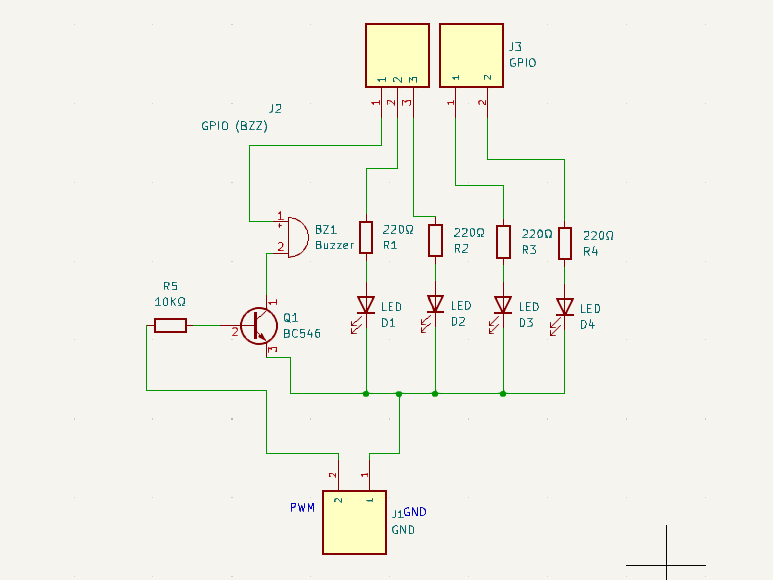
\includegraphics[width=1\textwidth]{Images/SistemaEmergencia/sistemergencia.png}
    \caption{Esquemático del sistema de emegencia}


    \begin{subfigure}[t]{0.5\textwidth}
        \centering
        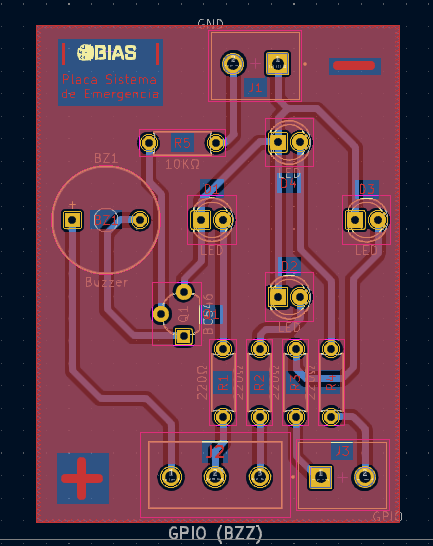
\includegraphics[width=0.75\textwidth]{Images/SistemaEmergencia/sistemergenciapcb.png}
        \caption{PCB Del sistema de emergencia}
    \end{subfigure}%
    ~ 
    \begin{subfigure}[t]{0.5\textwidth}
        \centering
        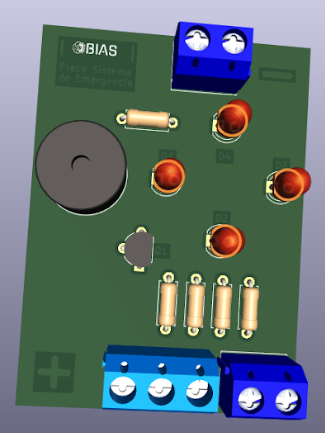
\includegraphics[width=0.75\textwidth]{Images/SistemaEmergencia/sistemergencia3d.png}
        \caption{Modelo 3D Del sistema de emergencia}
    \end{subfigure}

\end{figure}

\subsection{Lista de materiales}
Los programas desarrollados para el proyecto, tales como los filtros digitales, sistemas de inteligencia artificial y otros códigos relacionados, se almacenan en los siguientes dispositivos:

\begin{itemize}
    \item Raspberry Pi 4
    \item RP2040-zero
\end{itemize}

\subsubsection{EEG}
\begin{enumerate}
    \item TL084 (x4)
    \item AD620 (x8)
    \item Capacitores 100nF (x48)
    \item Resistencias 100Ω (x4)
    \item Resistencias 120Ω (x16)
    \item Resistencias 560Ω (x8) 
    \item Resistencias 820Ω (x16)
    \item Resistencias 1,5kΩ (x8)
    \item Resistencias 4,7kΩ (x16)
    \item Resistencias 12kΩ (x8)
    \item Resistencias 15kΩ (x8)
    \item Resistencias 27kΩ (x16)
    \item Resistencias 470kΩ (x8)
    \item Resistencias 2,7MΩ (x8)
    \item Electrodos (x9)
\end{enumerate}

\subsubsection{Placa OffSet}
\begin{enumerate}
    \item L7805 (x1)
    \item TL084 (x4)
    \item Jumpers (x2)
    \item Diodos Zenner 3,3V (x4)
    \item Capacitores 100nF (x4)
    \item Resistencias 220Ω (x4)
    \item Resistencias 50kΩ (x8)
    \item Resistencias 100kΩ (x8)
\end{enumerate}

\subsubsection{Sistema de Emergencia}
\begin{enumerate}
    \item Transistor BC546 (x1)
    \item Buzzer 5V (x1)
    \item LEDs Rojos (x4)
    \item Resistencias 220Ω (x4)
    \item Resistencia 4,7kΩ (x1)
\end{enumerate}

\subsubsection{Puentes H}
\begin{enumerate}
    \item Transistores IRF4905 (x4)
    \item Transistores IRF2805 (x4)
    \item Optoacopladores PC817 (x4)
    \item Motores 24V 575W (x2)
    \item Resistencias 100Ω (x4)
    \item Resistencias 180Ω (x4)
    \item Resistrencias 1kΩ (x4)
    \item Resistencias 4,7kΩ (x4)
\end{enumerate}

\subsubsection{Placa reguladora de tensión}
\begin{enumerate}
    \item LM7815 (x1)
    \item Capacitor 100μF (x1)
    \item Capacitor 330μF (x1)
    \item Capacitor 470μF 35V (x1)
    \item Capacitor 470μF 25V (x1)
\end{enumerate}

\section{Conclusiones}
En esta sección se presentará un análisis detallado de los conocimientos adquiridos a lo largo del desarrollo del proyecto, así como las conclusiones a las que hemos llegado durante este proceso. Se incluirán las conclusiones finales obtenidas, así como una evaluación de las principales limitaciones que afectaron el progreso del trabajo. Además, se ofrecerá un resumen de los resultados alcanzados, destacando los aspectos más relevantes y significativos. Finalmente, se abordarán las perspectivas futuras del proyecto, delineando los pasos a seguir para continuar su desarrollo y mejorarlo en el futuro.


\subsection{Resumen de Resultados}


\subsection{Limitaciones}
Durante la ejecución de este proyecto, nos enfrentamos a diversas limitaciones, algunas de las cuales fueron ocasionadas por circunstancias personales de cada integrante del equipo. Como es común en todo proyecto, al principio experimentamos dificultades en la organización y carecíamos de ciertos conocimientos técnicos, los cuales fuimos adquiriendo a lo largo del año.



El tiempo dedicado al proyecto quizá no fue suficiente, considerando la magnitud y la ambición del mismo. Además de estos desafíos iniciales, una de las principales limitaciones fue el prolongado tiempo de espera para obtener los materiales necesarios, los cuales provenían principalmente de la cooperadora. Dado que esta era nuestra principal fuente de herramientas y componentes, nuestro progreso estuvo estrictamente limitado por los tiempos de adquisición manejados por la institución.


Asimismo, al estar creando algo “nuevo”, nos vimos obligados a adoptar un enfoque basado en la prueba y error, ya que la información disponible sobre los temas específicos que requeríamos era escasa. Esta situación también representó un obstáculo significativo, ya que corregir nuestros errores consumió una parte considerable de nuestro tiempo.


Finalmente, al tratarse de un proyecto desarrollado en el ámbito escolar, también nos vimos limitados por el tiempo disponible en la escuela. No pudimos dedicar todo nuestro tiempo al proyecto, ya que debíamos atender otras asignaturas y compromisos académicos.

\subsection{Trabajo Futuro}
El proyecto presenta un alto potencial de rentabilidad en el futuro, sustentado en su carácter innovador y las posibilidades que ofrece su desarrollo continuo. Al tratarse de un invento único en su categoría, se prevé que, con el tiempo y el trabajo adicional necesario, este dispositivo pueda alcanzar un nivel de madurez suficiente para ser comercializado a gran escala.

La inversión en tiempo y recursos adicionales permitirá perfeccionar sus características técnicas, optimizar su funcionalidad, y adaptar el producto a las necesidades de un mercado en expansión. Una vez finalizado y refinado, el proyecto podrá captar la atención de un público más amplio, lo que incrementará su viabilidad comercial y su posicionamiento en el mercado.

En caso de que el desarrollo del proyecto no se complete en su totalidad, este podrá ser aprovechado por la institución educativa, permitiendo que otros grupos de estudiantes continúen su avance. De esta manera, el proyecto no solo servirá como un recurso valioso para futuras generaciones, sino que también fomentará la colaboración y el aprendizaje continuo dentro de la comunidad académica, garantizando su evolución y finalización.
\subsection {Informacion Adicional}
La silla desarrollada en este proyecto es un prototipo, es decir, puede contener fallas de todo tipo, y es sujeto a modificaciones a futuro. Se recomienda su uso siempre acompañado, en zonas amplias libres de obstáculos. No se debe usar en lugares húmedos o si el equipo está mojado, y la inteligencia artificial está adaptada a las muestras de una persona del equipo del proyecto, por lo que para ser usada por alguien mas se deberán muestrear los patrones de movimiento de esta misma.

\subsubsection{Programas Utilizados}
Para el desarrollo del proyecto, hemos requerido hacer uso de los siguientes porogramas, con sus enlaces principales: \newline


    \href{https://github.com/}{-Github}    
    \newline

    \href{https://code.visualstudio.com/}{-Visual Studio Code}
    \newline

    \href{https://thonny.org/}{-Thonny}
    \newline

    \href{https://es.overleaf.com/project}{-Overleaf}
    \newline

    \href{https://www.jetbrains.com/es-es/pycharm/}{-Pycharm}
    \newline

    \href{https://termius.com/}{-Termius}
    \newline

    \href{https://www.kicad.org/}{-Kicad}
    \newline

    \href{https://livewire.laravel.com/}{-Livewire}
    \newline

    \href{https://www.analog.com/en/resources/design-tools-and-calculators/ltspice-simulator.html}{-LTSpice}
    \newline

    \href{https://github.com/apps/desktop}{-GitHub Desktop}

\subsubsection{Agradecimientos}

Queremos expresar nuestro más profundo agradecimiento a los profesores que nos han brindado su invaluable apoyo en la realización de este proyecto:


Fabrizio Carlassara: Su asistencia fue crucial en la programación de la mayor parte del proyecto, así como en la creación de circuitos y esquemáticos, la búsqueda de materiales y el desarrollo de los filtros necesarios.


Sergio Medina: Nos brindó su experiencia en la presentación y comercialización del proyecto, además de colaborar en la programación, la búsqueda de materiales y la planificación de los puentes H.


Carlos Bianco: Su apoyo fue esencial en las pruebas y acondicionamiento de los motores, proporcionándonos herramientas y baterías para dichas pruebas, además de colaborar en la búsqueda de materiales.


Daniel Espósito: Nos proporcionó motores y materiales, además de enseñarnos a construir los puentes H para los motores, facilitando su creación y optimización.


Federico Solomiewicz: Su colaboración fue invaluable en el desarrollo de los filtros, proporcionándonos herramientas para el proyecto y estando siempre disponible para resolver cualquier duda que surgiera.


Juan Carlos Ruiz: Su colaboración fue esencial en las pruebas de los motores para la silla de ruedas, adempas de ayudarnos principalmente en la creación de los puentes H para los motores y sus circuitos impresos.



\section{Referencias}
En este apartado se presentarán de manera detallada las referencias consultadas al inicio del proyecto, las cuales fueron fundamentales para la conceptualización y desarrollo de la idea final. Estas fuentes proporcionaron el marco teórico y práctico necesario para orientar la dirección del trabajo, influyendo en las decisiones tomadas durante el proceso de diseño y ejecución.
\subsubsection{Autodesk Instructables}
A partir de esta página, obtuvimos los primeros circuitos necesarios para el EEG, lo que nos permitió avanzar de manera significativa en el desarrollo del proyecto. Esta fuente de información fue fundamental para sentar las bases técnicas y nos brindó las herramientas necesarias para continuar con el diseño y la implementación del sistema.


\section{Lista de códigos}

\subsection{Códigos principales}

\subsubsection{bias.py}
\lstinputlisting[language=python]{Codigos/CodigosPrincipales/bias.py}

\subsubsection{app.py}

\subsection{Inteligencia artificial}

\subsubsection{bias\_ai.py}

\subsection{Filtrado y procesamiento de señales}

\subsubsection{bias\_dsp.py}

\subsubsection{bias\_graphing.py} 
\lstinputlisting[language=python]{Codigos/Filtrado/bias_graphing.py}

\subsection{Motores}

\subsubsection{bias\_motors.py}
\lstinputlisting[language=python]{Codigos/Motores/bias_motors.py}

\subsection{Recepción de señales}

\subsubsection{bias\_reception.py}
\lstinputlisting[language=python]{Codigos/Recepcion/bias_reception.py}


\subsubsection{CMakeLists.txt}

\subsubsection{pico\_sdk\_import.cmake}

\subsubsection{reception.c}

\subsection{Página Web}
El sitio web ofrece una breve descripción sobre nosotros, nuestros objetivos, y proporciona enlaces a nuestras redes sociales, donde podrán contactarnos o conocer más acerca de nuestro trabajo.

\begin{center}
    \href{https://proyectobias.github.io/Bias/}{Página Web}
\end{center}

\subsubsection{Lenguaje utilizado en la página web y su código}
El desarrollo de la página web se realizó utilizando los lenguajes HTML y CSS.

Aquí se adjuntan los códigos de la página web:

\begin{center}
    Index.css
\end{center}

\lstinputlisting[language=CSS]{PaginaWeb/index.css}

\begin{center}
    Index.html
\end{center}

\lstinputlisting[language=html]{PaginaWeb/index.html}



\end{document}